\section*{Теоретические вопросы}

\subsection*{1. Элементы языка: определение, синтаксис, представление в памяти}

\subsubsection{Элементы языка}
Элементами языка {\texttt{Lisp}} являются атомы и точечные пары (структуры). К атомам относятся:
\begin{itemize}[topsep=0pt, noitemsep]
	\item символы (идентификаторы) -- набор литер, начинающихся с буквы;
	\item специальные символы для обозначения логических констант {\texttt{T,~Nil}};
	\item самоопределимые атомы -- натуральные числа, дробные числа, вещественные числа, строки (последовательность символов, заключённых в двойные апострофы).
\end{itemize}

\subsubsection*{Синтаксис элементов языка и их представление в памяти.}

\noindent{\texttt{Точечные пары ::= (<атом>, <атом>) |}}
{\texttt{(<атом>, <точечная пара>) |}}\\
{\texttt{(<точечная пара>, <атом>) |}}
{\texttt{(<точечная пара>, <точечная пара>)}}\\

\noindent{\texttt{Список ::= <пустой список> | <непустой список>)}}, где\\
{\texttt{<пустой список> ::= () | Nil}},\\
{\texttt{<непустой список> ::= (<первый элемент>, <хвост>) }},\\
{\texttt{<первый элемент> ::= (S-выражение)}},\\
{\texttt{<хвост> ::= <список>}}\\

\noindent Список -- частный случай {\texttt{S-выражения}}.\\
Синтаксически любая структура (точечная пара или список) заключается в {\texttt{()}}:\\
{\texttt{(A . B)}} -- точечная пара\\
{\texttt{(A)}} -- список из одного элемента\\
Пустой список изображается как {\texttt{Nil}} или {\texttt{()}}\\
Непустой список может быть изображён: {\texttt{(A. (B . (C ())))}} или {\texttt{(A B C)}}\\
Элементы списка могут являться списками: {\texttt{((A) (B) (C))}}\\
Любая непустая структура {\texttt{Lisp}} в памяти представлена списковой ячейкой, хранящей два указателя: на голову (первый элемент) и хвост (всё остальное).

\subsection*{2. Особенности языка LISP. Структура программы. Символ апостроф.}

\subsubsection*{Структура программы}

Lisp - язык символьной обработки. 
В Lisp программа и данные представлены списками.
По умолчанию список считается вычислимой формой, в которой 1 элемент - название функции, остальные элементы - аргументы функции.

\subsubsection*{Особенности языка}

Т.к. и программа и данные представлены списками, то их нужно как-то различать. 
Для этого была создана функция quote, а ' - ее сокращенное обозначение. 
quote - функция, блокирующая вычисление.

\subsubsection*{Символ апостроф}

Символ {\texttt{'}} -- функциональная блокировка, эквивалентен функции {\texttt{quote}}. Блокирует вычисление выражения. Таким образом, выражение воспринимается интерпретатором как данные.

\subsection*{3. Базис языка LISP. Ядро языка.}

Базис -- это минимальный набор инструментов языка и стркутур данных, который позволяет решить любые задачи.

Базис Lisp :

\begin{itemize}
	\item[$-$] атомы и структуры (представляющиеся бинарными узлами);
	\item[$-$] базовые (несколько) функций и функционалов: встроенные — примитивные 
	функции (atom, eq, cons, car, cdr); специальные функции и функционалы (quote, 
	cond, lambda, eval, apply, funcall).
\end{itemize}
	
Функцией называется правило, по которому каждому значению одного или нескольких  аргументов ставится в соответствие конкретное значение результата.

Функционалом, или функцией высшего порядка называется функция, аргументом или  результатом которой является другая функция.

Некоторые функции системы необходимо реализовывать в виде машинных подпрограмм, они образуют ядро системы. Ядро - основные действия, которые наиболее часто используются. Понятие <<ядро>> шире, чем понятие <<базис>>.

\section*{Практические задания}
\subsection*{Задание 1}

Представить следующие списки в виде списочных ячеек:
\begin{enumerate}[topsep=0pt]
	\item[$-$] {\texttt{'(open close halp)}}

	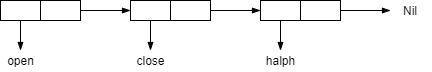
\includegraphics[scale=1]{img/1.1}

	\item[$-$] {\texttt{'((open1) (close2) (halp3))}}

	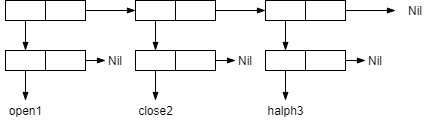
\includegraphics[scale=1]{img/1.2}

	\item[$-$] {\texttt{'((one) for all (and (me (for you))))}}

	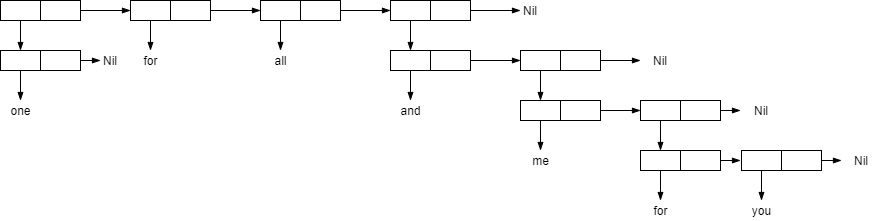
\includegraphics[scale=0.5]{img/1.3}
	\clearpage
	\item[$-$] {\texttt{'((TOOL) (call))}}
	
	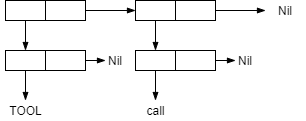
\includegraphics[scale=0.8]{img/1.4}

	\item[$-$] {\texttt{'((TOOL1) ((call2)) ((sell)))}}

	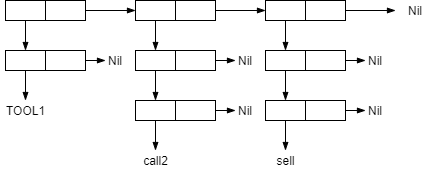
\includegraphics[scale=0.8]{img/1.5}

	\item[$-$] {\texttt{'(((TOOL) (call)) ((sell)))}}

	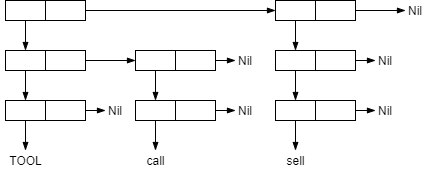
\includegraphics[scale=0.8]{img/1.6}
\end{enumerate}

\subsection*{Задание 2}

Используя только функции {\texttt{CAR}} и {\texttt{CDR}}, написать выражения, возвращающие второй, третий, четвёртый элементы заданного списка:

\begin{lstinputlisting}[
	label={lst:t1},
	style={lsp},
	linerange={3-10},
	]{../src/main.lsp}
\end{lstinputlisting}

\subsection*{Задание 3}

Что будет в результате выполнения выражений?

\begin{lstinputlisting}[
	label={lst:t2},
	style={lsp},
	linerange={14-17},
	]{../src/main.lsp}
\end{lstinputlisting}

\subsection*{Задание 4}

Напишите результат вычисления выражений:

\begin{lstinputlisting}[
	label={lst:t3},
	style={lsp},
	linerange={19-35},
	]{../src/main.lsp}
\end{lstinputlisting}

\subsection*{Задание 5}

Написать лямбда-выражение и соответствующую функцию. Представить результаты в виде списочных ячеек.

\begin{itemize}[topsep=0pt, noitemsep]
	\item[$-$] Написать функцию (f arl ar2 ar3 ar4), возвращающую список \\((arl ar2) (ar3 ar4)).
	\begin{lstinputlisting}[
		label={lst:t4},
		style={lsp},
		linerange={38-42},
		]{../src/main.lsp}
	\end{lstinputlisting}
	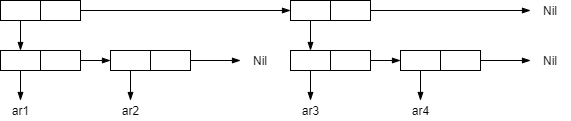
\includegraphics[scale=0.7]{img/1}

	\item[$-$] Написать функцию (f arl ar2), возвращающую ((arl) (ar2))
	\begin{lstinputlisting}[
		label={lst:t4},
		style={lsp},
		linerange={44-48},
		]{../src/main.lsp}
	\end{lstinputlisting}
	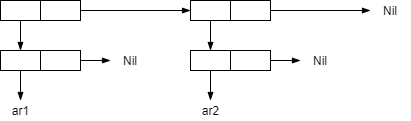
\includegraphics[scale=0.7]{img/2}

	\item[$-$] Написать функцию (f arl), возвращающую (((arl))).
	\begin{lstinputlisting}[
		label={lst:t4},
		style={lsp},
		linerange={50-54},
		]{../src/main.lsp}
	\end{lstinputlisting}
	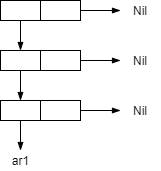
\includegraphics[scale=0.7]{img/3}

\end{itemize}

